\documentclass[1p]{elsarticle_modified}
%\bibliographystyle{elsarticle-num}

%\usepackage[colorlinks]{hyperref}
%\usepackage{abbrmath_seonhwa} %\Abb, \Ascr, \Acal ,\Abf, \Afrak
\usepackage{amsfonts}
\usepackage{amssymb}
\usepackage{amsmath}
\usepackage{amsthm}
\usepackage{scalefnt}
\usepackage{amsbsy}
\usepackage{kotex}
\usepackage{caption}
\usepackage{subfig}
\usepackage{color}
\usepackage{graphicx}
\usepackage{xcolor} %% white, black, red, green, blue, cyan, magenta, yellow
\usepackage{float}
\usepackage{setspace}
\usepackage{hyperref}

\usepackage{tikz}
\usetikzlibrary{arrows}

\usepackage{multirow}
\usepackage{array} % fixed length table
\usepackage{hhline}

%%%%%%%%%%%%%%%%%%%%%
\makeatletter
\renewcommand*\env@matrix[1][\arraystretch]{%
	\edef\arraystretch{#1}%
	\hskip -\arraycolsep
	\let\@ifnextchar\new@ifnextchar
	\array{*\c@MaxMatrixCols c}}
\makeatother %https://tex.stackexchange.com/questions/14071/how-can-i-increase-the-line-spacing-in-a-matrix
%%%%%%%%%%%%%%%

\usepackage[normalem]{ulem}

\newcommand{\msout}[1]{\ifmmode\text{\sout{\ensuremath{#1}}}\else\sout{#1}\fi}
%SOURCE: \msout is \stkout macro in https://tex.stackexchange.com/questions/20609/strikeout-in-math-mode

\newcommand{\cancel}[1]{
	\ifmmode
	{\color{red}\msout{#1}}
	\else
	{\color{red}\sout{#1}}
	\fi
}

\newcommand{\add}[1]{
	{\color{blue}\uwave{#1}}
}

\newcommand{\replace}[2]{
	\ifmmode
	{\color{red}\msout{#1}}{\color{blue}\uwave{#2}}
	\else
	{\color{red}\sout{#1}}{\color{blue}\uwave{#2}}
	\fi
}

\newcommand{\Sol}{\mathcal{S}} %segment
\newcommand{\D}{D} %diagram
\newcommand{\A}{\mathcal{A}} %arc


%%%%%%%%%%%%%%%%%%%%%%%%%%%%%5 test

\def\sl{\operatorname{\textup{SL}}(2,\Cbb)}
\def\psl{\operatorname{\textup{PSL}}(2,\Cbb)}
\def\quan{\mkern 1mu \triangleright \mkern 1mu}

\theoremstyle{definition}
\newtheorem{thm}{Theorem}[section]
\newtheorem{prop}[thm]{Proposition}
\newtheorem{lem}[thm]{Lemma}
\newtheorem{ques}[thm]{Question}
\newtheorem{cor}[thm]{Corollary}
\newtheorem{defn}[thm]{Definition}
\newtheorem{exam}[thm]{Example}
\newtheorem{rmk}[thm]{Remark}
\newtheorem{alg}[thm]{Algorithm}

\newcommand{\I}{\sqrt{-1}}
\begin{document}

%\begin{frontmatter}
%
%\title{Boundary parabolic representations of knots up to 8 crossings}
%
%%% Group authors per affiliation:
%\author{Yunhi Cho} 
%\address{Department of Mathematics, University of Seoul, Seoul, Korea}
%\ead{yhcho@uos.ac.kr}
%
%
%\author{Seonhwa Kim} %\fnref{s_kim}}
%\address{Center for Geometry and Physics, Institute for Basic Science, Pohang, 37673, Korea}
%\ead{ryeona17@ibs.re.kr}
%
%\author{Hyuk Kim}
%\address{Department of Mathematical Sciences, Seoul National University, Seoul 08826, Korea}
%\ead{hyukkim@snu.ac.kr}
%
%\author{Seokbeom Yoon}
%\address{Department of Mathematical Sciences, Seoul National University, Seoul, 08826,  Korea}
%\ead{sbyoon15@snu.ac.kr}
%
%\begin{abstract}
%We find all boundary parabolic representation of knots up to 8 crossings.
%
%\end{abstract}
%\begin{keyword}
%    \MSC[2010] 57M25 
%\end{keyword}
%
%\end{frontmatter}

%\linenumbers
%\tableofcontents
%
\newcommand\colored[1]{\textcolor{white}{\rule[-0.35ex]{0.8em}{1.4ex}}\kern-0.8em\color{red} #1}%
%\newcommand\colored[1]{\textcolor{white}{ #1}\kern-2.17ex	\textcolor{white}{ #1}\kern-1.81ex	\textcolor{white}{ #1}\kern-2.15ex\color{red}#1	}

{\Large $\underline{11a_{139}~(K11a_{139})}$}

\setlength{\tabcolsep}{10pt}
\renewcommand{\arraystretch}{1.6}
\vspace{1cm}\begin{tabular}{m{100pt}>{\centering\arraybackslash}m{274pt}}
\multirow{5}{120pt}{
	\centering
	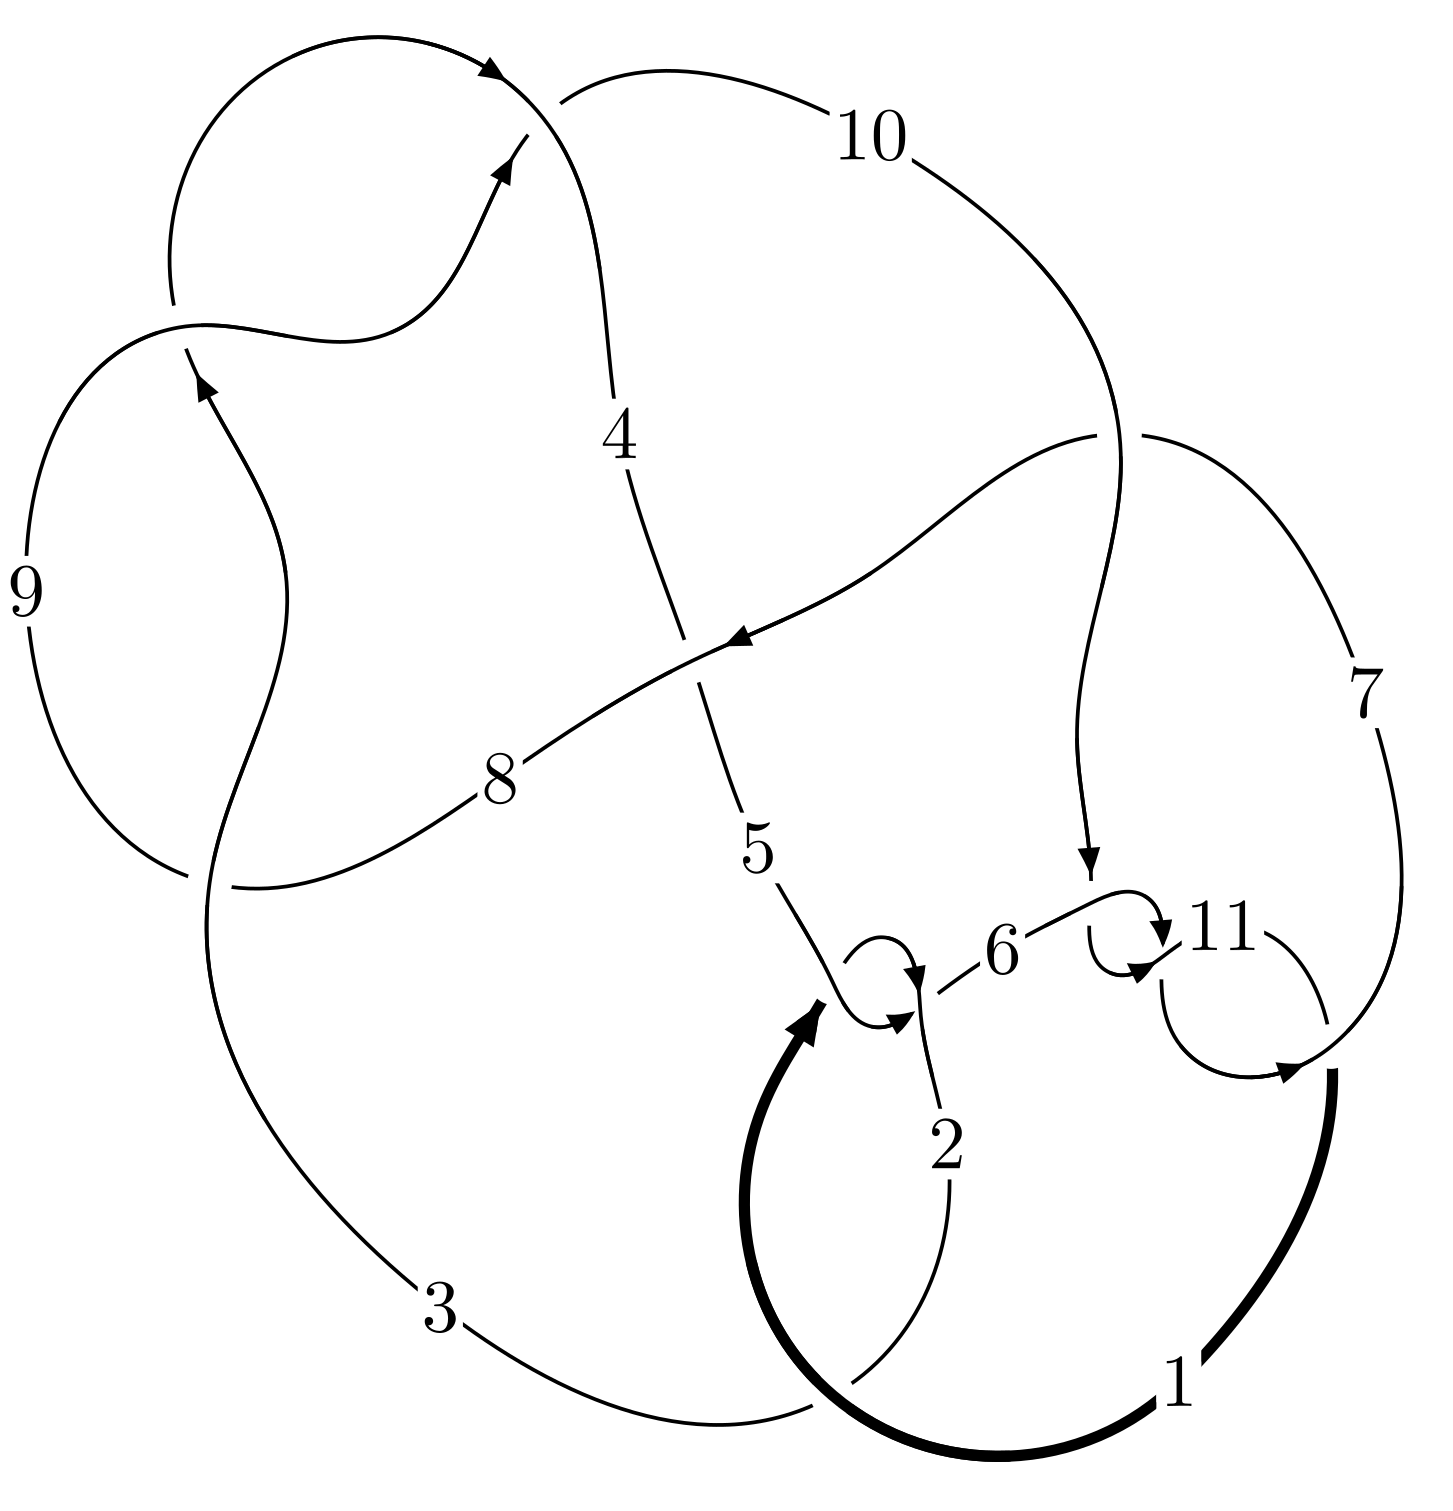
\includegraphics[width=112pt]{../../../GIT/diagram.site/Diagrams/png/388_11a_139.png}\\
\ \ \ A knot diagram\footnotemark}&
\allowdisplaybreaks
\textbf{Linearized knot diagam} \\
\cline{2-2}
 &
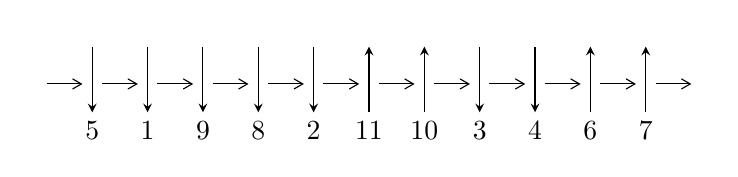
\begin{tikzpicture}[x=20pt, y=17pt]
	% nodes
	\node (C0) at (0, 0) {};
	\node (C1) at (1, 0) {};
	\node (C1U) at (1, +1) {};
	\node (C1D) at (1, -1) {5};

	\node (C2) at (2, 0) {};
	\node (C2U) at (2, +1) {};
	\node (C2D) at (2, -1) {1};

	\node (C3) at (3, 0) {};
	\node (C3U) at (3, +1) {};
	\node (C3D) at (3, -1) {9};

	\node (C4) at (4, 0) {};
	\node (C4U) at (4, +1) {};
	\node (C4D) at (4, -1) {8};

	\node (C5) at (5, 0) {};
	\node (C5U) at (5, +1) {};
	\node (C5D) at (5, -1) {2};

	\node (C6) at (6, 0) {};
	\node (C6U) at (6, +1) {};
	\node (C6D) at (6, -1) {11};

	\node (C7) at (7, 0) {};
	\node (C7U) at (7, +1) {};
	\node (C7D) at (7, -1) {10};

	\node (C8) at (8, 0) {};
	\node (C8U) at (8, +1) {};
	\node (C8D) at (8, -1) {3};

	\node (C9) at (9, 0) {};
	\node (C9U) at (9, +1) {};
	\node (C9D) at (9, -1) {4};

	\node (C10) at (10, 0) {};
	\node (C10U) at (10, +1) {};
	\node (C10D) at (10, -1) {6};

	\node (C11) at (11, 0) {};
	\node (C11U) at (11, +1) {};
	\node (C11D) at (11, -1) {7};
	\node (C12) at (12, 0) {};

	% arrows
	\draw[->,>={angle 60}]
	(C0) edge (C1) (C1) edge (C2) (C2) edge (C3) (C3) edge (C4) (C4) edge (C5) (C5) edge (C6) (C6) edge (C7) (C7) edge (C8) (C8) edge (C9) (C9) edge (C10) (C10) edge (C11) (C11) edge (C12) ;	\draw[->,>=stealth]
	(C1U) edge (C1D) (C2U) edge (C2D) (C3U) edge (C3D) (C4U) edge (C4D) (C5U) edge (C5D) (C6D) edge (C6U) (C7D) edge (C7U) (C8U) edge (C8D) (C9U) edge (C9D) (C10D) edge (C10U) (C11D) edge (C11U) ;
	\end{tikzpicture} \\
\hhline{~~} \\& 
\textbf{Solving Sequence} \\ \cline{2-2} 
 &
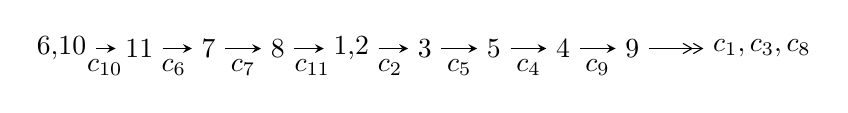
\begin{tikzpicture}[x=25pt, y=7pt]
	% node
	\node (A0) at (-1/8, 0) {6,10};
	\node (A1) at (1, 0) {11};
	\node (A2) at (2, 0) {7};
	\node (A3) at (3, 0) {8};
	\node (A4) at (65/16, 0) {1,2};
	\node (A5) at (41/8, 0) {3};
	\node (A6) at (49/8, 0) {5};
	\node (A7) at (57/8, 0) {4};
	\node (A8) at (65/8, 0) {9};
	\node (C1) at (1/2, -1) {$c_{10}$};
	\node (C2) at (3/2, -1) {$c_{6}$};
	\node (C3) at (5/2, -1) {$c_{7}$};
	\node (C4) at (7/2, -1) {$c_{11}$};
	\node (C5) at (37/8, -1) {$c_{2}$};
	\node (C6) at (45/8, -1) {$c_{5}$};
	\node (C7) at (53/8, -1) {$c_{4}$};
	\node (C8) at (61/8, -1) {$c_{9}$};
	\node (A9) at (10, 0) {$c_{1},c_{3},c_{8}$};

	% edge
	\draw[->,>=stealth]	
	(A0) edge (A1) (A1) edge (A2) (A2) edge (A3) (A3) edge (A4) (A4) edge (A5) (A5) edge (A6) (A6) edge (A7) (A7) edge (A8) ;
	\draw[->>,>={angle 60}]	
	(A8) edge (A9);
\end{tikzpicture} \\ 

\end{tabular} \\

\footnotetext{
The image of knot diagram is generated by the software ``\textbf{Draw programme}" developed by Andrew Bartholomew(\url{http://www.layer8.co.uk/maths/draw/index.htm\#Running-draw}), where we modified some parts for our purpose(\url{https://github.com/CATsTAILs/LinksPainter}).
}\phantom \\ \newline 
\centering \textbf{Ideals for irreducible components\footnotemark of $X_{\text{par}}$} 
 
\begin{align*}
I^u_{1}&=\langle 
-1330328 u^{36}-337157 u^{35}+\cdots+3064546 b-5423429,\\
\phantom{I^u_{1}}&\phantom{= \langle  }2108869 u^{36}-5518964 u^{35}+\cdots+1532273 a+24842943,\;u^{37}-2 u^{36}+\cdots+13 u+1\rangle \\
I^u_{2}&=\langle 
u^2+b,\;a-1,\;u^{15}-5 u^{13}- u^{12}+10 u^{11}+4 u^{10}-8 u^9-6 u^8- u^7+3 u^6+5 u^5+u^4- u^3- u^2- u-1\rangle \\
I^u_{3}&=\langle 
b^2+2 b-1,\;a-1,\;u+1\rangle \\
I^u_{4}&=\langle 
b+1,\;a-1,\;u-1\rangle \\
\\
\end{align*}
\raggedright * 4 irreducible components of $\dim_{\mathbb{C}}=0$, with total 55 representations.\\
\footnotetext{All coefficients of polynomials are rational numbers. But the coefficients are sometimes approximated in decimal forms when there is not enough margin.}
\newpage
\renewcommand{\arraystretch}{1}
\centering \section*{I. $I^u_{1}= \langle -1.33\times10^{6} u^{36}-3.37\times10^{5} u^{35}+\cdots+3.06\times10^{6} b-5.42\times10^{6},\;2.11\times10^{6} u^{36}-5.52\times10^{6} u^{35}+\cdots+1.53\times10^{6} a+2.48\times10^{7},\;u^{37}-2 u^{36}+\cdots+13 u+1 \rangle$}
\flushleft \textbf{(i) Arc colorings}\\
\begin{tabular}{m{7pt} m{180pt} m{7pt} m{180pt} }
\flushright $a_{6}=$&$\begin{pmatrix}0\\u\end{pmatrix}$ \\
\flushright $a_{10}=$&$\begin{pmatrix}1\\0\end{pmatrix}$ \\
\flushright $a_{11}=$&$\begin{pmatrix}1\\- u^2\end{pmatrix}$ \\
\flushright $a_{7}=$&$\begin{pmatrix}u\\- u^3+u\end{pmatrix}$ \\
\flushright $a_{8}=$&$\begin{pmatrix}- u^3+2 u\\- u^3+u\end{pmatrix}$ \\
\flushright $a_{1}=$&$\begin{pmatrix}- u^2+1\\u^4-2 u^2\end{pmatrix}$ \\
\flushright $a_{2}=$&$\begin{pmatrix}-1.37630 u^{36}+3.60182 u^{35}+\cdots-53.4414 u-16.2131\\0.434103 u^{36}+0.110019 u^{35}+\cdots+4.77936 u+1.76973\end{pmatrix}$ \\
\flushright $a_{3}=$&$\begin{pmatrix}-1.61129 u^{36}+4.21702 u^{35}+\cdots-52.0448 u-17.2627\\-1.20630 u^{36}+0.913862 u^{35}+\cdots+17.4922 u+2.71463\end{pmatrix}$ \\
\flushright $a_{5}=$&$\begin{pmatrix}-1.84921 u^{36}+3.03426 u^{35}+\cdots-28.6788 u-14.3763\\-0.129011 u^{36}-0.605251 u^{35}+\cdots+4.55239 u+1.81040\end{pmatrix}$ \\
\flushright $a_{4}=$&$\begin{pmatrix}-1.03926 u^{36}+2.83241 u^{35}+\cdots-37.3538 u-14.7413\\-0.817794 u^{36}+0.142729 u^{35}+\cdots+14.2739 u+2.65174\end{pmatrix}$ \\
\flushright $a_{9}=$&$\begin{pmatrix}1.35408 u^{36}-3.76576 u^{35}+\cdots+69.5409 u+23.2930\\0.656314 u^{36}+0.203071 u^{35}+\cdots-15.2619 u-3.27106\end{pmatrix}$\\ \flushright $a_{9}=$&$\begin{pmatrix}1.35408 u^{36}-3.76576 u^{35}+\cdots+69.5409 u+23.2930\\0.656314 u^{36}+0.203071 u^{35}+\cdots-15.2619 u-3.27106\end{pmatrix}$\\&\end{tabular}
\flushleft \textbf{(ii) Obstruction class $= -1$}\\~\\
\flushleft \textbf{(iii) Cusp Shapes $= -\frac{5839087}{1532273} u^{36}+\frac{3620132}{1532273} u^{35}+\cdots+\frac{36237593}{1532273} u-\frac{19224398}{1532273}$}\\~\\
\newpage\renewcommand{\arraystretch}{1}
\flushleft \textbf{(iv) u-Polynomials at the component}\newline \\
\begin{tabular}{m{50pt}|m{274pt}}
Crossings & \hspace{64pt}u-Polynomials at each crossing \\
\hline $$\begin{aligned}c_{1},c_{5}\end{aligned}$$&$\begin{aligned}
&u^{37}+2 u^{36}+\cdots+u+1
\end{aligned}$\\
\hline $$\begin{aligned}c_{2}\end{aligned}$$&$\begin{aligned}
&u^{37}+18 u^{36}+\cdots+5 u+1
\end{aligned}$\\
\hline $$\begin{aligned}c_{3},c_{8},c_{9}\end{aligned}$$&$\begin{aligned}
&u^{37}+2 u^{36}+\cdots+2 u^2-2
\end{aligned}$\\
\hline $$\begin{aligned}c_{4}\end{aligned}$$&$\begin{aligned}
&u^{37}-6 u^{36}+\cdots+288 u-128
\end{aligned}$\\
\hline $$\begin{aligned}c_{6},c_{10},c_{11}\end{aligned}$$&$\begin{aligned}
&u^{37}-2 u^{36}+\cdots+13 u+1
\end{aligned}$\\
\hline $$\begin{aligned}c_{7}\end{aligned}$$&$\begin{aligned}
&u^{37}+6 u^{36}+\cdots-224 u-16
\end{aligned}$\\
\hline
\end{tabular}\\~\\
\newpage\renewcommand{\arraystretch}{1}
\flushleft \textbf{(v) Riley Polynomials at the component}\newline \\
\begin{tabular}{m{50pt}|m{274pt}}
Crossings & \hspace{64pt}Riley Polynomials at each crossing \\
\hline $$\begin{aligned}c_{1},c_{5}\end{aligned}$$&$\begin{aligned}
&y^{37}-18 y^{36}+\cdots+5 y-1
\end{aligned}$\\
\hline $$\begin{aligned}c_{2}\end{aligned}$$&$\begin{aligned}
&y^{37}+6 y^{36}+\cdots+21 y-1
\end{aligned}$\\
\hline $$\begin{aligned}c_{3},c_{8},c_{9}\end{aligned}$$&$\begin{aligned}
&y^{37}-34 y^{36}+\cdots+8 y-4
\end{aligned}$\\
\hline $$\begin{aligned}c_{4}\end{aligned}$$&$\begin{aligned}
&y^{37}-10 y^{36}+\cdots+156672 y-16384
\end{aligned}$\\
\hline $$\begin{aligned}c_{6},c_{10},c_{11}\end{aligned}$$&$\begin{aligned}
&y^{37}-34 y^{36}+\cdots+117 y-1
\end{aligned}$\\
\hline $$\begin{aligned}c_{7}\end{aligned}$$&$\begin{aligned}
&y^{37}+18 y^{36}+\cdots+32256 y-256
\end{aligned}$\\
\hline
\end{tabular}\\~\\
\newpage\flushleft \textbf{(vi) Complex Volumes and Cusp Shapes}
$$\begin{array}{c|c|c}  
\text{Solutions to }I^u_{1}& \I (\text{vol} + \sqrt{-1}CS) & \text{Cusp shape}\\
 \hline 
\begin{aligned}
u &= -1.013380 + 0.311874 I \\
a &= -0.007083 + 0.507321 I \\
b &= -0.911372 + 0.339991 I\end{aligned}
 & -3.23840 + 0.33679 I & -3.19033 + 0.85162 I \\ \hline\begin{aligned}
u &= -1.013380 - 0.311874 I \\
a &= -0.007083 - 0.507321 I \\
b &= -0.911372 - 0.339991 I\end{aligned}
 & -3.23840 - 0.33679 I & -3.19033 - 0.85162 I \\ \hline\begin{aligned}
u &= -0.148500 + 0.878352 I \\
a &= -0.35212 + 1.40071 I \\
b &= -0.17334 + 2.13411 I\end{aligned}
 & -8.84281 - 9.20717 I & -9.51764 + 6.62975 I \\ \hline\begin{aligned}
u &= -0.148500 - 0.878352 I \\
a &= -0.35212 - 1.40071 I \\
b &= -0.17334 - 2.13411 I\end{aligned}
 & -8.84281 + 9.20717 I & -9.51764 - 6.62975 I \\ \hline\begin{aligned}
u &= -1.15117\phantom{ +0.000000I} \\
a &= -0.432099\phantom{ +0.000000I} \\
b &= -1.94913\phantom{ +0.000000I}\end{aligned}
 & -3.47854\phantom{ +0.000000I} & -0.910990\phantom{ +0.000000I} \\ \hline\begin{aligned}
u &= \phantom{-}0.165281 + 0.808869 I \\
a &= -0.30320 - 1.46229 I \\
b &= -0.11222 - 1.95034 I\end{aligned}
 & -3.03568 + 5.84417 I & -5.83954 - 7.10655 I \\ \hline\begin{aligned}
u &= \phantom{-}0.165281 - 0.808869 I \\
a &= -0.30320 + 1.46229 I \\
b &= -0.11222 + 1.95034 I\end{aligned}
 & -3.03568 - 5.84417 I & -5.83954 + 7.10655 I \\ \hline\begin{aligned}
u &= -0.471583 + 0.599168 I \\
a &= \phantom{-}0.162338 + 1.262080 I \\
b &= -0.480709 + 1.121580 I\end{aligned}
 & -2.94289 - 4.00123 I & -5.31382 + 7.13651 I \\ \hline\begin{aligned}
u &= -0.471583 - 0.599168 I \\
a &= \phantom{-}0.162338 - 1.262080 I \\
b &= -0.480709 - 1.121580 I\end{aligned}
 & -2.94289 + 4.00123 I & -5.31382 - 7.13651 I \\ \hline\begin{aligned}
u &= -0.022041 + 0.744033 I \\
a &= -0.53343 - 1.59774 I \\
b &= \phantom{-}0.42055 - 2.05462 I\end{aligned}
 & -9.93818 - 0.58603 I & -11.65035 - 0.12880 I\\
 \hline 
 \end{array}$$\newpage$$\begin{array}{c|c|c}  
\text{Solutions to }I^u_{1}& \I (\text{vol} + \sqrt{-1}CS) & \text{Cusp shape}\\
 \hline 
\begin{aligned}
u &= -0.022041 - 0.744033 I \\
a &= -0.53343 + 1.59774 I \\
b &= \phantom{-}0.42055 + 2.05462 I\end{aligned}
 & -9.93818 + 0.58603 I & -11.65035 + 0.12880 I \\ \hline\begin{aligned}
u &= -0.099912 + 0.709675 I \\
a &= -0.33485 + 1.62744 I \\
b &= \phantom{-}0.17353 + 1.80893 I\end{aligned}
 & -3.65380 - 1.92705 I & -8.13048 + 0.55620 I \\ \hline\begin{aligned}
u &= -0.099912 - 0.709675 I \\
a &= -0.33485 - 1.62744 I \\
b &= \phantom{-}0.17353 - 1.80893 I\end{aligned}
 & -3.65380 + 1.92705 I & -8.13048 - 0.55620 I \\ \hline\begin{aligned}
u &= -1.253160 + 0.303469 I \\
a &= -0.759003 - 0.531242 I \\
b &= \phantom{-}1.10971 - 2.91416 I\end{aligned}
 & -6.13830 - 3.19514 I & -6.64446 + 4.28023 I \\ \hline\begin{aligned}
u &= -1.253160 - 0.303469 I \\
a &= -0.759003 + 0.531242 I \\
b &= \phantom{-}1.10971 + 2.91416 I\end{aligned}
 & -6.13830 + 3.19514 I & -6.64446 - 4.28023 I \\ \hline\begin{aligned}
u &= \phantom{-}1.296560 + 0.177192 I \\
a &= -0.331390 - 0.464636 I \\
b &= -0.683956 - 0.483013 I\end{aligned}
 & \phantom{-}3.08964 + 0.95760 I & \phantom{-0.000000 -}     -6
0. 10   + 1.305195 I \\ \hline\begin{aligned}
u &= \phantom{-}1.296560 - 0.177192 I \\
a &= -0.331390 + 0.464636 I \\
b &= -0.683956 + 0.483013 I\end{aligned}
 & \phantom{-}3.08964 - 0.95760 I & \phantom{-0.000000 }      -6
0. 10   - 1.305195 I \\ \hline\begin{aligned}
u &= \phantom{-}0.568431 + 0.375314 I \\
a &= \phantom{-}0.520054 - 0.971540 I \\
b &= -0.443456 - 0.641882 I\end{aligned}
 & \phantom{-}0.89372 + 1.45212 I & \phantom{-}2.19487 - 5.36999 I \\ \hline\begin{aligned}
u &= \phantom{-}0.568431 - 0.375314 I \\
a &= \phantom{-}0.520054 + 0.971540 I \\
b &= -0.443456 + 0.641882 I\end{aligned}
 & \phantom{-}0.89372 - 1.45212 I & \phantom{-}2.19487 + 5.36999 I \\ \hline\begin{aligned}
u &= \phantom{-}1.332640 + 0.298347 I \\
a &= -0.706159 + 0.554504 I \\
b &= \phantom{-}1.13989 + 2.44217 I\end{aligned}
 & \phantom{-}0.86122 + 5.58916 I & -3.00000 - 3.15563 I\\
 \hline 
 \end{array}$$\newpage$$\begin{array}{c|c|c}  
\text{Solutions to }I^u_{1}& \I (\text{vol} + \sqrt{-1}CS) & \text{Cusp shape}\\
 \hline 
\begin{aligned}
u &= \phantom{-}1.332640 - 0.298347 I \\
a &= -0.706159 - 0.554504 I \\
b &= \phantom{-}1.13989 - 2.44217 I\end{aligned}
 & \phantom{-}0.86122 - 5.58916 I & -3.00000 + 3.15563 I \\ \hline\begin{aligned}
u &= -1.350860 + 0.271610 I \\
a &= -0.313821 + 0.546709 I \\
b &= -0.634567 + 0.232909 I\end{aligned}
 & \phantom{-}4.43467 - 4.86040 I & \phantom{-0.000000 -}0. + 4.57417 I \\ \hline\begin{aligned}
u &= -1.350860 - 0.271610 I \\
a &= -0.313821 - 0.546709 I \\
b &= -0.634567 - 0.232909 I\end{aligned}
 & \phantom{-}4.43467 + 4.86040 I & \phantom{-0.000000 } 0. - 4.57417 I \\ \hline\begin{aligned}
u &= \phantom{-}1.361180 + 0.332115 I \\
a &= -0.298381 - 0.581807 I \\
b &= -0.695184 - 0.117059 I\end{aligned}
 & -1.06880 + 8.43099 I & \phantom{-0.000000 } 0. - 5.07593 I \\ \hline\begin{aligned}
u &= \phantom{-}1.361180 - 0.332115 I \\
a &= -0.298381 + 0.581807 I \\
b &= -0.695184 + 0.117059 I\end{aligned}
 & -1.06880 - 8.43099 I & \phantom{-0.000000 -}0. + 5.07593 I \\ \hline\begin{aligned}
u &= \phantom{-}1.400590 + 0.045310 I \\
a &= -0.466611 - 0.492889 I \\
b &= -0.170732 - 0.843883 I\end{aligned}
 & \phantom{-}3.96621 + 1.16950 I & \phantom{-0.000000 } 0 \\ \hline\begin{aligned}
u &= \phantom{-}1.400590 - 0.045310 I \\
a &= -0.466611 + 0.492889 I \\
b &= -0.170732 + 0.843883 I\end{aligned}
 & \phantom{-}3.96621 - 1.16950 I & \phantom{-0.000000 } 0 \\ \hline\begin{aligned}
u &= -1.366970 + 0.343185 I \\
a &= -0.701831 - 0.589074 I \\
b &= \phantom{-}1.41347 - 2.32983 I\end{aligned}
 & \phantom{-}1.80064 - 9.99903 I & \phantom{-0.000000 -}0. + 8.15131 I \\ \hline\begin{aligned}
u &= -1.366970 - 0.343185 I \\
a &= -0.701831 + 0.589074 I \\
b &= \phantom{-}1.41347 + 2.32983 I\end{aligned}
 & \phantom{-}1.80064 + 9.99903 I & \phantom{-0.000000 } 0. - 8.15131 I \\ \hline\begin{aligned}
u &= -1.411670 + 0.052360 I \\
a &= -0.537001 - 0.501630 I \\
b &= \phantom{-}0.155713 - 1.234020 I\end{aligned}
 & \phantom{-}7.20025 - 2.58398 I & \phantom{-}4.12642 + 3.46228 I\\
 \hline 
 \end{array}$$\newpage$$\begin{array}{c|c|c}  
\text{Solutions to }I^u_{1}& \I (\text{vol} + \sqrt{-1}CS) & \text{Cusp shape}\\
 \hline 
\begin{aligned}
u &= -1.411670 - 0.052360 I \\
a &= -0.537001 + 0.501630 I \\
b &= \phantom{-}0.155713 + 1.234020 I\end{aligned}
 & \phantom{-}7.20025 + 2.58398 I & \phantom{-}4.12642 - 3.46228 I \\ \hline\begin{aligned}
u &= \phantom{-}1.37052 + 0.38186 I \\
a &= -0.709680 + 0.609188 I \\
b &= \phantom{-}1.59214 + 2.36282 I\end{aligned}
 & -4.0535 + 13.7305 I & \phantom{-0.000000 } 0. - 8.23789 I \\ \hline\begin{aligned}
u &= \phantom{-}1.37052 - 0.38186 I \\
a &= -0.709680 - 0.609188 I \\
b &= \phantom{-}1.59214 - 2.36282 I\end{aligned}
 & -4.0535 - 13.7305 I & \phantom{-0.000000 -}0. + 8.23789 I \\ \hline\begin{aligned}
u &= \phantom{-}1.41824 + 0.13440 I \\
a &= -0.588434 + 0.523307 I \\
b &= \phantom{-}0.51535 + 1.54249 I\end{aligned}
 & \phantom{-}3.18948 + 6.36871 I & \phantom{-0.000000 } 0. - 6.27419 I \\ \hline\begin{aligned}
u &= \phantom{-}1.41824 - 0.13440 I \\
a &= -0.588434 - 0.523307 I \\
b &= \phantom{-}0.51535 - 1.54249 I\end{aligned}
 & \phantom{-}3.18948 - 6.36871 I & \phantom{-0.000000 -}0. + 6.27419 I \\ \hline\begin{aligned}
u &= -0.302230\phantom{ +0.000000I} \\
a &= \phantom{-}2.69339\phantom{ +0.000000I} \\
b &= \phantom{-}0.212469\phantom{ +0.000000I}\end{aligned}
 & -1.08012\phantom{ +0.000000I} & -10.9510\phantom{ +0.000000I} \\ \hline\begin{aligned}
u &= -0.0973082\phantom{ +0.000000I} \\
a &= -10.7401\phantom{ +0.000000I} \\
b &= \phantom{-}1.30703\phantom{ +0.000000I}\end{aligned}
 & -6.54639\phantom{ +0.000000I} & -13.9600\phantom{ +0.000000I}\\
 \hline 
 \end{array}$$\newpage\newpage\renewcommand{\arraystretch}{1}
\centering \section*{II. $I^u_{2}= \langle u^2+b,\;a-1,\;u^{15}-5 u^{13}+\cdots- u-1 \rangle$}
\flushleft \textbf{(i) Arc colorings}\\
\begin{tabular}{m{7pt} m{180pt} m{7pt} m{180pt} }
\flushright $a_{6}=$&$\begin{pmatrix}0\\u\end{pmatrix}$ \\
\flushright $a_{10}=$&$\begin{pmatrix}1\\0\end{pmatrix}$ \\
\flushright $a_{11}=$&$\begin{pmatrix}1\\- u^2\end{pmatrix}$ \\
\flushright $a_{7}=$&$\begin{pmatrix}u\\- u^3+u\end{pmatrix}$ \\
\flushright $a_{8}=$&$\begin{pmatrix}- u^3+2 u\\- u^3+u\end{pmatrix}$ \\
\flushright $a_{1}=$&$\begin{pmatrix}- u^2+1\\u^4-2 u^2\end{pmatrix}$ \\
\flushright $a_{2}=$&$\begin{pmatrix}1\\- u^2\end{pmatrix}$ \\
\flushright $a_{3}=$&$\begin{pmatrix}u^4- u^2+1\\- u^6+2 u^4- u^2\end{pmatrix}$ \\
\flushright $a_{5}=$&$\begin{pmatrix}u\\- u^3+u\end{pmatrix}$ \\
\flushright $a_{4}=$&$\begin{pmatrix}- u^9+4 u^7-5 u^5+2 u^3+u\\- u^9+3 u^7-3 u^5+u\end{pmatrix}$ \\
\flushright $a_{9}=$&$\begin{pmatrix}u^{13}-4 u^{11}+7 u^9-6 u^7+2 u^5+u\\- u^{12}+4 u^{10}+u^9-6 u^8-3 u^7+3 u^6+3 u^5+u^4- u^3- u^2-1\end{pmatrix}$\\ \flushright $a_{9}=$&$\begin{pmatrix}u^{13}-4 u^{11}+7 u^9-6 u^7+2 u^5+u\\- u^{12}+4 u^{10}+u^9-6 u^8-3 u^7+3 u^6+3 u^5+u^4- u^3- u^2-1\end{pmatrix}$\\&\end{tabular}
\flushleft \textbf{(ii) Obstruction class $= -1$}\\~\\
\flushleft \textbf{(iii) Cusp Shapes $= 4 u^9-12 u^7-4 u^6+12 u^5+8 u^4-4 u^2-4 u-6$}\\~\\
\newpage\renewcommand{\arraystretch}{1}
\flushleft \textbf{(iv) u-Polynomials at the component}\newline \\
\begin{tabular}{m{50pt}|m{274pt}}
Crossings & \hspace{64pt}u-Polynomials at each crossing \\
\hline $$\begin{aligned}c_{1},c_{5},c_{6}\\c_{10},c_{11}\end{aligned}$$&$\begin{aligned}
&u^{15}-5 u^{13}+\cdots- u-1
\end{aligned}$\\
\hline $$\begin{aligned}c_{2}\end{aligned}$$&$\begin{aligned}
&u^{15}+10 u^{14}+\cdots- u+1
\end{aligned}$\\
\hline $$\begin{aligned}c_{3},c_{8},c_{9}\end{aligned}$$&$\begin{aligned}
&(u^5- u^4-2 u^3+u^2+u+1)^3
\end{aligned}$\\
\hline $$\begin{aligned}c_{4}\end{aligned}$$&$\begin{aligned}
&(u^5+3 u^4+4 u^3+u^2- u-1)^3
\end{aligned}$\\
\hline $$\begin{aligned}c_{7}\end{aligned}$$&$\begin{aligned}
&(u^5+u^4+2 u^3+u^2+u+1)^3
\end{aligned}$\\
\hline
\end{tabular}\\~\\
\newpage\renewcommand{\arraystretch}{1}
\flushleft \textbf{(v) Riley Polynomials at the component}\newline \\
\begin{tabular}{m{50pt}|m{274pt}}
Crossings & \hspace{64pt}Riley Polynomials at each crossing \\
\hline $$\begin{aligned}c_{1},c_{5},c_{6}\\c_{10},c_{11}\end{aligned}$$&$\begin{aligned}
&y^{15}-10 y^{14}+\cdots- y-1
\end{aligned}$\\
\hline $$\begin{aligned}c_{2}\end{aligned}$$&$\begin{aligned}
&y^{15}-10 y^{14}+\cdots+7 y-1
\end{aligned}$\\
\hline $$\begin{aligned}c_{3},c_{8},c_{9}\end{aligned}$$&$\begin{aligned}
&(y^5-5 y^4+8 y^3-3 y^2- y-1)^3
\end{aligned}$\\
\hline $$\begin{aligned}c_{4}\end{aligned}$$&$\begin{aligned}
&(y^5- y^4+8 y^3-3 y^2+3 y-1)^3
\end{aligned}$\\
\hline $$\begin{aligned}c_{7}\end{aligned}$$&$\begin{aligned}
&(y^5+3 y^4+4 y^3+y^2- y-1)^3
\end{aligned}$\\
\hline
\end{tabular}\\~\\
\newpage\flushleft \textbf{(vi) Complex Volumes and Cusp Shapes}
$$\begin{array}{c|c|c}  
\text{Solutions to }I^u_{2}& \I (\text{vol} + \sqrt{-1}CS) & \text{Cusp shape}\\
 \hline 
\begin{aligned}
u &= \phantom{-}1.051760 + 0.377982 I \\
a &= \phantom{-}1.00000\phantom{ +0.000000I} \\
b &= -0.963319 - 0.795090 I\end{aligned}
 & -0.32910 - 1.53058 I & -2.51511 + 4.43065 I \\ \hline\begin{aligned}
u &= \phantom{-}1.051760 - 0.377982 I \\
a &= \phantom{-}1.00000\phantom{ +0.000000I} \\
b &= -0.963319 + 0.795090 I\end{aligned}
 & -0.32910 + 1.53058 I & -2.51511 - 4.43065 I \\ \hline\begin{aligned}
u &= -0.162112 + 0.782578 I \\
a &= \phantom{-}1.00000\phantom{ +0.000000I} \\
b &= \phantom{-}0.586148 + 0.253730 I\end{aligned}
 & -5.87256 - 4.40083 I & -6.74431 + 3.49859 I \\ \hline\begin{aligned}
u &= -0.162112 - 0.782578 I \\
a &= \phantom{-}1.00000\phantom{ +0.000000I} \\
b &= \phantom{-}0.586148 - 0.253730 I\end{aligned}
 & -5.87256 + 4.40083 I & -6.74431 - 3.49859 I \\ \hline\begin{aligned}
u &= -1.121390 + 0.470419 I \\
a &= \phantom{-}1.00000\phantom{ +0.000000I} \\
b &= -1.03622 + 1.05504 I\end{aligned}
 & -5.87256 + 4.40083 I & -6.74431 - 3.49859 I \\ \hline\begin{aligned}
u &= -1.121390 - 0.470419 I \\
a &= \phantom{-}1.00000\phantom{ +0.000000I} \\
b &= -1.03622 - 1.05504 I\end{aligned}
 & -5.87256 - 4.40083 I & -6.74431 + 3.49859 I \\ \hline\begin{aligned}
u &= -0.633490 + 0.451585 I \\
a &= \phantom{-}1.00000\phantom{ +0.000000I} \\
b &= -0.197381 + 0.572150 I\end{aligned}
 & -2.40108\phantom{ +0.000000I} & -3.48114 + 0. I\phantom{ +0.000000I} \\ \hline\begin{aligned}
u &= -0.633490 - 0.451585 I \\
a &= \phantom{-}1.00000\phantom{ +0.000000I} \\
b &= -0.197381 - 0.572150 I\end{aligned}
 & -2.40108\phantom{ +0.000000I} & -3.48114 + 0. I\phantom{ +0.000000I} \\ \hline\begin{aligned}
u &= -1.209710 + 0.247023 I \\
a &= \phantom{-}1.00000\phantom{ +0.000000I} \\
b &= -1.40237 + 0.59765 I\end{aligned}
 & -0.32910 - 1.53058 I & -2.51511 + 4.43065 I \\ \hline\begin{aligned}
u &= -1.209710 - 0.247023 I \\
a &= \phantom{-}1.00000\phantom{ +0.000000I} \\
b &= -1.40237 - 0.59765 I\end{aligned}
 & -0.32910 + 1.53058 I & -2.51511 - 4.43065 I\\
 \hline 
 \end{array}$$\newpage$$\begin{array}{c|c|c}  
\text{Solutions to }I^u_{2}& \I (\text{vol} + \sqrt{-1}CS) & \text{Cusp shape}\\
 \hline 
\begin{aligned}
u &= \phantom{-}1.26698\phantom{ +0.000000I} \\
a &= \phantom{-}1.00000\phantom{ +0.000000I} \\
b &= -1.60524\phantom{ +0.000000I}\end{aligned}
 & -2.40108\phantom{ +0.000000I} & -3.48110\phantom{ +0.000000I} \\ \hline\begin{aligned}
u &= \phantom{-}1.283500 + 0.312159 I \\
a &= \phantom{-}1.00000\phantom{ +0.000000I} \\
b &= -1.54993 - 0.80131 I\end{aligned}
 & -5.87256 + 4.40083 I & -6.74431 - 3.49859 I \\ \hline\begin{aligned}
u &= \phantom{-}1.283500 - 0.312159 I \\
a &= \phantom{-}1.00000\phantom{ +0.000000I} \\
b &= -1.54993 + 0.80131 I\end{aligned}
 & -5.87256 - 4.40083 I & -6.74431 + 3.49859 I \\ \hline\begin{aligned}
u &= \phantom{-}0.157950 + 0.625006 I \\
a &= \phantom{-}1.00000\phantom{ +0.000000I} \\
b &= \phantom{-}0.365684 - 0.197439 I\end{aligned}
 & -0.32910 + 1.53058 I & -2.51511 - 4.43065 I \\ \hline\begin{aligned}
u &= \phantom{-}0.157950 - 0.625006 I \\
a &= \phantom{-}1.00000\phantom{ +0.000000I} \\
b &= \phantom{-}0.365684 + 0.197439 I\end{aligned}
 & -0.32910 - 1.53058 I & -2.51511 + 4.43065 I\\
 \hline 
 \end{array}$$\newpage\newpage\renewcommand{\arraystretch}{1}
\centering \section*{III. $I^u_{3}= \langle b^2+2 b-1,\;a-1,\;u+1 \rangle$}
\flushleft \textbf{(i) Arc colorings}\\
\begin{tabular}{m{7pt} m{180pt} m{7pt} m{180pt} }
\flushright $a_{6}=$&$\begin{pmatrix}0\\-1\end{pmatrix}$ \\
\flushright $a_{10}=$&$\begin{pmatrix}1\\0\end{pmatrix}$ \\
\flushright $a_{11}=$&$\begin{pmatrix}1\\-1\end{pmatrix}$ \\
\flushright $a_{7}=$&$\begin{pmatrix}-1\\0\end{pmatrix}$ \\
\flushright $a_{8}=$&$\begin{pmatrix}-1\\0\end{pmatrix}$ \\
\flushright $a_{1}=$&$\begin{pmatrix}0\\-1\end{pmatrix}$ \\
\flushright $a_{2}=$&$\begin{pmatrix}1\\b\end{pmatrix}$ \\
\flushright $a_{3}=$&$\begin{pmatrix}1\\b+1\end{pmatrix}$ \\
\flushright $a_{5}=$&$\begin{pmatrix}-1\\- b-1\end{pmatrix}$ \\
\flushright $a_{4}=$&$\begin{pmatrix}- b-2\\- b-1\end{pmatrix}$ \\
\flushright $a_{9}=$&$\begin{pmatrix}- b-2\\-2\end{pmatrix}$\\ \flushright $a_{9}=$&$\begin{pmatrix}- b-2\\-2\end{pmatrix}$\\&\end{tabular}
\flushleft \textbf{(ii) Obstruction class $= 1$}\\~\\
\flushleft \textbf{(iii) Cusp Shapes $= -8$}\\~\\
\newpage\renewcommand{\arraystretch}{1}
\flushleft \textbf{(iv) u-Polynomials at the component}\newline \\
\begin{tabular}{m{50pt}|m{274pt}}
Crossings & \hspace{64pt}u-Polynomials at each crossing \\
\hline $$\begin{aligned}c_{1},c_{2},c_{10}\\c_{11}\end{aligned}$$&$\begin{aligned}
&(u+1)^2
\end{aligned}$\\
\hline $$\begin{aligned}c_{3},c_{4},c_{8}\\c_{9}\end{aligned}$$&$\begin{aligned}
&u^2-2
\end{aligned}$\\
\hline $$\begin{aligned}c_{5},c_{6}\end{aligned}$$&$\begin{aligned}
&(u-1)^2
\end{aligned}$\\
\hline $$\begin{aligned}c_{7}\end{aligned}$$&$\begin{aligned}
&u^2
\end{aligned}$\\
\hline
\end{tabular}\\~\\
\newpage\renewcommand{\arraystretch}{1}
\flushleft \textbf{(v) Riley Polynomials at the component}\newline \\
\begin{tabular}{m{50pt}|m{274pt}}
Crossings & \hspace{64pt}Riley Polynomials at each crossing \\
\hline $$\begin{aligned}c_{1},c_{2},c_{5}\\c_{6},c_{10},c_{11}\end{aligned}$$&$\begin{aligned}
&(y-1)^2
\end{aligned}$\\
\hline $$\begin{aligned}c_{3},c_{4},c_{8}\\c_{9}\end{aligned}$$&$\begin{aligned}
&(y-2)^2
\end{aligned}$\\
\hline $$\begin{aligned}c_{7}\end{aligned}$$&$\begin{aligned}
&y^2
\end{aligned}$\\
\hline
\end{tabular}\\~\\
\newpage\flushleft \textbf{(vi) Complex Volumes and Cusp Shapes}
$$\begin{array}{c|c|c}  
\text{Solutions to }I^u_{3}& \I (\text{vol} + \sqrt{-1}CS) & \text{Cusp shape}\\
 \hline 
\begin{aligned}
u &= -1.00000\phantom{ +0.000000I} \\
a &= \phantom{-}1.00000\phantom{ +0.000000I} \\
b &= \phantom{-}0.414214\phantom{ +0.000000I}\end{aligned}
 & -4.93480\phantom{ +0.000000I} & -8.00000\phantom{ +0.000000I} \\ \hline\begin{aligned}
u &= -1.00000\phantom{ +0.000000I} \\
a &= \phantom{-}1.00000\phantom{ +0.000000I} \\
b &= -2.41421\phantom{ +0.000000I}\end{aligned}
 & -4.93480\phantom{ +0.000000I} & -8.00000\phantom{ +0.000000I}\\
 \hline 
 \end{array}$$\newpage\newpage\renewcommand{\arraystretch}{1}
\centering \section*{IV. $I^u_{4}= \langle b+1,\;a-1,\;u-1 \rangle$}
\flushleft \textbf{(i) Arc colorings}\\
\begin{tabular}{m{7pt} m{180pt} m{7pt} m{180pt} }
\flushright $a_{6}=$&$\begin{pmatrix}0\\1\end{pmatrix}$ \\
\flushright $a_{10}=$&$\begin{pmatrix}1\\0\end{pmatrix}$ \\
\flushright $a_{11}=$&$\begin{pmatrix}1\\-1\end{pmatrix}$ \\
\flushright $a_{7}=$&$\begin{pmatrix}1\\0\end{pmatrix}$ \\
\flushright $a_{8}=$&$\begin{pmatrix}1\\0\end{pmatrix}$ \\
\flushright $a_{1}=$&$\begin{pmatrix}0\\-1\end{pmatrix}$ \\
\flushright $a_{2}=$&$\begin{pmatrix}1\\-1\end{pmatrix}$ \\
\flushright $a_{3}=$&$\begin{pmatrix}1\\0\end{pmatrix}$ \\
\flushright $a_{5}=$&$\begin{pmatrix}1\\0\end{pmatrix}$ \\
\flushright $a_{4}=$&$\begin{pmatrix}1\\0\end{pmatrix}$ \\
\flushright $a_{9}=$&$\begin{pmatrix}1\\0\end{pmatrix}$\\ \flushright $a_{9}=$&$\begin{pmatrix}1\\0\end{pmatrix}$\\&\end{tabular}
\flushleft \textbf{(ii) Obstruction class $= 1$}\\~\\
\flushleft \textbf{(iii) Cusp Shapes $= 0$}\\~\\
\newpage\renewcommand{\arraystretch}{1}
\flushleft \textbf{(iv) u-Polynomials at the component}\newline \\
\begin{tabular}{m{50pt}|m{274pt}}
Crossings & \hspace{64pt}u-Polynomials at each crossing \\
\hline $$\begin{aligned}c_{1},c_{10},c_{11}\end{aligned}$$&$\begin{aligned}
&u-1
\end{aligned}$\\
\hline $$\begin{aligned}c_{2},c_{5},c_{6}\end{aligned}$$&$\begin{aligned}
&u+1
\end{aligned}$\\
\hline $$\begin{aligned}c_{3},c_{4},c_{7}\\c_{8},c_{9}\end{aligned}$$&$\begin{aligned}
&u
\end{aligned}$\\
\hline
\end{tabular}\\~\\
\newpage\renewcommand{\arraystretch}{1}
\flushleft \textbf{(v) Riley Polynomials at the component}\newline \\
\begin{tabular}{m{50pt}|m{274pt}}
Crossings & \hspace{64pt}Riley Polynomials at each crossing \\
\hline $$\begin{aligned}c_{1},c_{2},c_{5}\\c_{6},c_{10},c_{11}\end{aligned}$$&$\begin{aligned}
&y-1
\end{aligned}$\\
\hline $$\begin{aligned}c_{3},c_{4},c_{7}\\c_{8},c_{9}\end{aligned}$$&$\begin{aligned}
&y
\end{aligned}$\\
\hline
\end{tabular}\\~\\
\newpage\flushleft \textbf{(vi) Complex Volumes and Cusp Shapes}
$$\begin{array}{c|c|c}  
\text{Solutions to }I^u_{4}& \I (\text{vol} + \sqrt{-1}CS) & \text{Cusp shape}\\
 \hline 
\begin{aligned}
u &= \phantom{-}1.00000\phantom{ +0.000000I} \\
a &= \phantom{-}1.00000\phantom{ +0.000000I} \\
b &= -1.00000\phantom{ +0.000000I}\end{aligned}
 & \phantom{-0.000000 } 0 & \phantom{-0.000000 } 0\\
 \hline 
 \end{array}$$\newpage
\newpage\renewcommand{\arraystretch}{1}
\centering \section*{ V. u-Polynomials}
\begin{tabular}{m{50pt}|m{274pt}}
Crossings & \hspace{64pt}u-Polynomials at each crossing \\
\hline $$\begin{aligned}c_{1}\end{aligned}$$&$\begin{aligned}
&(u-1)(u+1)^2(u^{15}-5 u^{13}+\cdots- u-1)(u^{37}+2 u^{36}+\cdots+u+1)
\end{aligned}$\\
\hline $$\begin{aligned}c_{2}\end{aligned}$$&$\begin{aligned}
&((u+1)^3)(u^{15}+10 u^{14}+\cdots- u+1)(u^{37}+18 u^{36}+\cdots+5 u+1)
\end{aligned}$\\
\hline $$\begin{aligned}c_{3},c_{8},c_{9}\end{aligned}$$&$\begin{aligned}
&u(u^2-2)(u^5- u^4+\cdots+u+1)^{3}(u^{37}+2 u^{36}+\cdots+2 u^{2}-2)
\end{aligned}$\\
\hline $$\begin{aligned}c_{4}\end{aligned}$$&$\begin{aligned}
&u(u^2-2)(u^5+3 u^4+\cdots- u-1)^{3}(u^{37}-6 u^{36}+\cdots+288 u-128)
\end{aligned}$\\
\hline $$\begin{aligned}c_{5}\end{aligned}$$&$\begin{aligned}
&((u-1)^2)(u+1)(u^{15}-5 u^{13}+\cdots- u-1)(u^{37}+2 u^{36}+\cdots+u+1)
\end{aligned}$\\
\hline $$\begin{aligned}c_{6}\end{aligned}$$&$\begin{aligned}
&((u-1)^2)(u+1)(u^{15}-5 u^{13}+\cdots- u-1)(u^{37}-2 u^{36}+\cdots+13 u+1)
\end{aligned}$\\
\hline $$\begin{aligned}c_{7}\end{aligned}$$&$\begin{aligned}
&u^3(u^5+u^4+\cdots+u+1)^{3}(u^{37}+6 u^{36}+\cdots-224 u-16)
\end{aligned}$\\
\hline $$\begin{aligned}c_{10},c_{11}\end{aligned}$$&$\begin{aligned}
&(u-1)(u+1)^2(u^{15}-5 u^{13}+\cdots- u-1)(u^{37}-2 u^{36}+\cdots+13 u+1)
\end{aligned}$\\
\hline
\end{tabular}\newpage\renewcommand{\arraystretch}{1}
\centering \section*{ VI. Riley Polynomials}
\begin{tabular}{m{50pt}|m{274pt}}
Crossings & \hspace{64pt}Riley Polynomials at each crossing \\
\hline $$\begin{aligned}c_{1},c_{5}\end{aligned}$$&$\begin{aligned}
&((y-1)^3)(y^{15}-10 y^{14}+\cdots- y-1)(y^{37}-18 y^{36}+\cdots+5 y-1)
\end{aligned}$\\
\hline $$\begin{aligned}c_{2}\end{aligned}$$&$\begin{aligned}
&((y-1)^3)(y^{15}-10 y^{14}+\cdots+7 y-1)(y^{37}+6 y^{36}+\cdots+21 y-1)
\end{aligned}$\\
\hline $$\begin{aligned}c_{3},c_{8},c_{9}\end{aligned}$$&$\begin{aligned}
&y(y-2)^2(y^5-5 y^4+\cdots- y-1)^{3}(y^{37}-34 y^{36}+\cdots+8 y-4)
\end{aligned}$\\
\hline $$\begin{aligned}c_{4}\end{aligned}$$&$\begin{aligned}
&y(y-2)^2(y^5- y^4+8 y^3-3 y^2+3 y-1)^3\\
&\cdot(y^{37}-10 y^{36}+\cdots+156672 y-16384)
\end{aligned}$\\
\hline $$\begin{aligned}c_{6},c_{10},c_{11}\end{aligned}$$&$\begin{aligned}
&((y-1)^3)(y^{15}-10 y^{14}+\cdots- y-1)(y^{37}-34 y^{36}+\cdots+117 y-1)
\end{aligned}$\\
\hline $$\begin{aligned}c_{7}\end{aligned}$$&$\begin{aligned}
&y^3(y^5+3 y^4+\cdots- y-1)^{3}(y^{37}+18 y^{36}+\cdots+32256 y-256)
\end{aligned}$\\
\hline
\end{tabular}
\vskip 2pc
\end{document}